%%%%%%%%%%%%%%%%%%%%%%%%%%%%%%%%%%%%%%%%%%%%%%
% Head matter - can we try to be consistent on
% included packages
\documentclass{beamer}
\mode<presentation>
{\usetheme{default}
 \usecolortheme{default}
 \usefonttheme{default}
 \setbeamertemplate{navigation symbols}{}
 \setbeamertemplate{footline}[frame number]
% \setbeamertemplate{caption}[numbered]
 }
\usepackage[english]{babel}
\usepackage{algorithm}
\usepackage[noend]{algpseudocode}
\usepackage[utf8x]{inputenc}
\usepackage{graphicx}
\usepackage{hyperref}
%\graphicspath{{./images/}}
\usepackage{tikz}
\usetikzlibrary{shapes.geometric, arrows,chains}
\usepackage{booktabs,makecell,multirow,tabularx}
\usepackage{verbatim}
\renewcommand{\arraystretch}{1.2}
\renewcommand\theadfont{\normalfont\bfseries}
\usepackage{array}
\usepackage{listings}
\lstset{language=Java, showstringspaces=false}
\usepackage[normalem]{ulem}
\usepackage{bm}
\def\layersep{2.5cm}

\usepackage{xcolor}
%\usepackage{subfig}
\setbeamertemplate{caption}{\insertcaption}
\usepackage[caption=false]{subfig}
\usepackage{hyperref}
\usepackage{verbatim}
%\setbeamertemplate{caption}[numbered]%\numberwithin{figure}{section}
% Define block styles
\tikzstyle{decision} = [diamond, draw, fill=blue!20, 
    text width=4.5em, text badly centered, node distance=3cm, inner sep=0pt]
\tikzstyle{block} = [rectangle, draw, fill=blue!20, 
    text width=3em, text centered, rounded corners, minimum height=3em]
\tikzstyle{line} = [draw, -latex']
\tikzstyle{cloud} = [draw, ellipse, fill=red!20, node distance=3cm,
    minimum height=2em]
\tikzset{
  startstop/.style={
    rectangle, 
    rounded corners,
    minimum width=3cm, 
    minimum height=1cm,
    align=center, 
    draw=black, 
    fill=red!30
    },
  process/.style={
    rectangle, 
    minimum width=3cm, 
    minimum height=1cm, 
    align=center, 
    draw=black, 
    fill=blue!30
    },
  decision/.style={
    rectangle, 
    minimum width=3cm, 
    minimum height=1cm, align=center, 
    draw=black, 
    fill=green!30
    },
  arrow/.style={thick,->,>=stealth},
  dec/.style={
    ellipse, 
    align=center, 
    draw=black, 
    fill=green!30
    },
}
\tikzstyle{arrow} = [thick,->,>=stealth]

\tikzset{onslide/.code args={<#1>#2}{%
  \only<#1>{\pgfkeysalso{#2}} % \pgfkeysalso doesn't change the path
}}

\makeatletter
\newenvironment<>{btHighlight}[1][]
{\begin{onlyenv}#2\begingroup\tikzset{bt@Highlight@par/.style={#1}}\begin{lrbox}{\@tempboxa}}
{\end{lrbox}\bt@HL@box[bt@Highlight@par]{\@tempboxa}\endgroup\end{onlyenv}}

\newcommand<>\btHL[1][]{%
  \only#2{\begin{btHighlight}[#1]\bgroup\aftergroup\bt@HL@endenv}%
}
\def\bt@HL@endenv{%
  \end{btHighlight}%   
  \egroup
}
\newcommand{\bt@HL@box}[2][]{%
  \tikz[#1]{%
    \pgfpathrectangle{\pgfpoint{1pt}{0pt}}{\pgfpoint{\wd #2}{\ht #2}}%
    \pgfusepath{use as bounding box}%
    \node[anchor=base west, fill=orange!30,outer sep=0pt,inner xsep=1pt, inner ysep=0pt, rounded corners=3pt, minimum height=\ht\strutbox+1pt,#1]{\raisebox{1pt}{\strut}\strut\usebox{#2}};
  }%
}
\makeatother




%%%%%%%%%%%%%%%%%%%%%%%%%%%%%%%%%%%%%%%%%%%%%%
% Formatting for title page
\title[Deep Learning]{Solving Deeper Multilayer Perceptrons (MLPs)}
\author{Kate Farrahi}
\institute{ECS Southampton} 
\date{\today}
%%%%%%%%%%%%%%%%%%%%%%%%%%%%%%%%%%%%%%%%%%%%%%
\begin{document}
\begin{frame}
  \titlepage \footnote{Some of this lecture has been motivated by F. Fleuret's course EE-559 at EPFL.}
\end{frame}



\begin{frame}{pause}\frametitle{What is Vectorization?}
\begin{itemize}
\item Vectorization helps improve the speed of your code by removing for loops \pause
\item The idea is that we want to apply a function to every element in a vector \pause
\item The activation of the $j$th neuron in the $l$th layer is given by 
\begin{equation}
a_j^l = \sigma(\sum_k w_{jk}^l a_k^{l-1} + b_j^l) \label{eqn:nonvect}
\end{equation} \pause
\item The model parameters can be represented in a matrix form by defining a weight matrix $w^l$ for each layer, $l$ and a bias vector, $b^l$ \pause
\item Vectorization can simplify our notation $a^l = \sigma(w^l a^{l-1} + b^l)$ 
\end{itemize}
\end{frame}
%-------------------------------------------------------------%
%
%\begin{frame}{pause}\frametitle{What is Vectorization?}
%\begin{itemize}
%\item Let us introduce the {\em weighted input} term, $z^l$, where $z^l = w^l a^{l-1} + b^l$ \pause
%\item Let's assume the MSE cost function $J = \frac{1}{2M}\sum_x (y(x) - a^L(x) )^2$ \pause
%\item Note, $a^L = \hat y$, but we will use $a$ in our derivation since we need to keep track of outputs over intermediary neurons.
%\end{itemize}
%\end{frame}

%%-------------------------------------------------------------%
\begin{frame}[fragile]\frametitle{Threshold Logic Unit}

The first mathematical model for a neuron was the Threshold Logic Unit, with
Boolean inputs and outputs:
\begin{equation}
f (x) = 1_{\{ w \sum_i x_i + b \geq 0 \} }
\end{equation}
 
In particular it can implement \\
\vspace{2mm}
$or(u, v) = 1_{\{ u + v - 0.5 \geq 0 \} }$ \hspace{4mm}  $(w = 1, b = -0.5)$ \\ 
$and(u, v) = 1_{\{ u + v - 1.5 \geq 0 \} }$ \hspace{3mm}  $(w = 1, b = -1.5)$ \\ 
$not(u) = 1_{\{ -u + 0.5 \geq 0 \} }$ \hspace{8mm}  $(w = -1, b = 0.5)$ \footnote{W. S. McCulloch and W. Pitts. A logical calculus of the ideas immanent in nervous activity. The bulletin of mathematical biophysics, 5(4):115-133, 1943}
\end{frame}

%-------------------------------------------------------------%
\begin{frame}[fragile]\frametitle{Perceptron}

The perceptron is very similar

\[  f(x) = \Bigg \{
  \begin{tabular}{ccc}
  $1$ & \text{if} & $\sum_i w_i x_i + b \geq 0 $ \\
  $0$ &  & \text{otherwise} \\
  \end{tabular}
\]
\\ \vspace{1 mm}
but the inputs are real values and the weights can be different. \\ \vspace{1 mm}
This model was originally motivated by biology, with $w_i$ being the synaptic
weights, and $x_i$ and $f$ firing rates. \\ \vspace{1 mm}
It is a (very) crude biological model. \footnote{F. Rosenblatt. The perceptron: A perceiving and recognizing automaton. Technical Report 85-460-1, Cornell Aeronautical Laboratory, 1957.}
\end{frame}

%-------------------------------------------------------------%

\begin{frame}[fragile]\frametitle{Perceptron}
\center{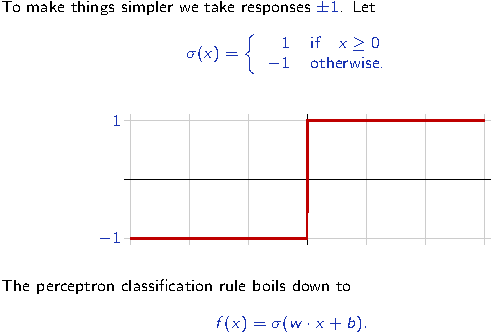
\includegraphics[width=0.8\textwidth]{perceptron.pdf}} 
%The perceptron rule boils down to
%
%\begin{equation}
%f(x) = \sigma (w  x + b)
%\end{equation}
%
%For neural networks the function $\sigma$ that follows the linear operation is  the activation function.
\end{frame}
%-------------------------------------------------------------%


\begin{frame}[fragile]\frametitle{Neuron}
\center{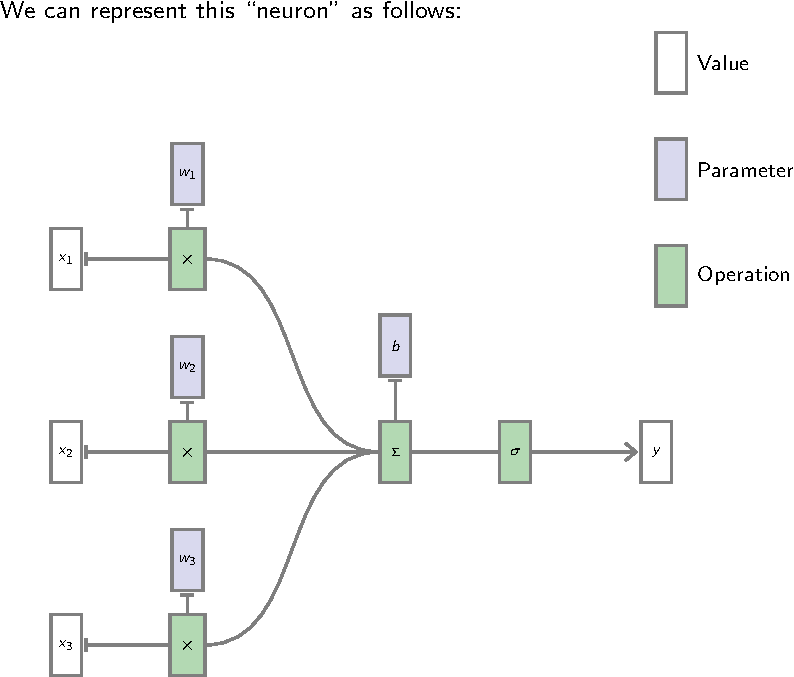
\includegraphics[width=0.8\textwidth]{neuron.pdf}} 
\end{frame}
%-------------------------------------------------------------%

\begin{frame}[fragile]\frametitle{Vectorized Perceptron Model}
\center{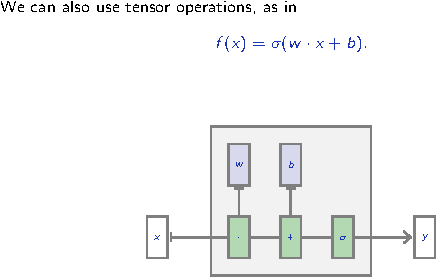
\includegraphics[width=0.8\textwidth]{perceptron_tensor.pdf}} 
\end{frame}
%-------------------------------------------------------------%

\begin{frame}[fragile]\frametitle{Learning Rule}
\center{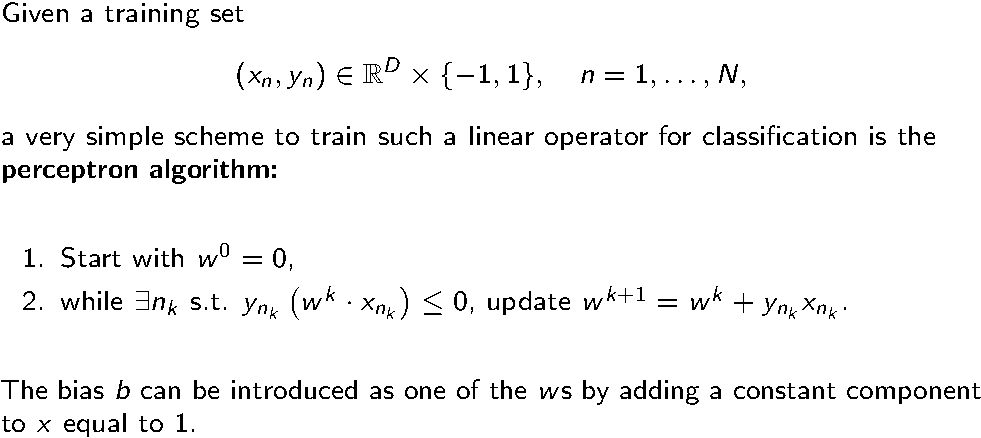
\includegraphics[width=0.8\textwidth]{rosenblatt.pdf}}
\end{frame}
%-------------------------------------------------------------%


%\begin{frame}[fragile]\frametitle{Perceptron Convergence Theorem}
%\url{http://hagan.okstate.edu/4_Perceptron.pdf }
%\end{frame}
%-------------------------------------------------------------%


%\begin{frame}[fragile]\frametitle{Perceptron}
%Final points about perceptron. \\
%- Each neuron finds a decision boundary \\
%- Some of the functions it can't learn (Figure 4.6 of \url{http://hagan.okstate.edu/4_Perceptron.pdf }) \\
%- The multiple-neuron perceptron
%\end{frame}
%%-------------------------------------------------------------%

\begin{frame}[fragile]\frametitle{Multilayer Perceptrons}
\center{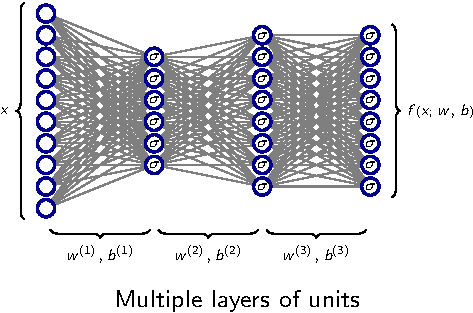
\includegraphics[width=0.9\textwidth]{DNN.pdf}} 
\end{frame}
%-------------------------------------------------------------%


\begin{frame}[fragile]\frametitle{Multilayer Perceptron (MLP)}

We can define the MLP formally as, \\ \vspace{0.5cm}

$\forall l = 1, 2, \dots, L, \hspace{1cm} a^{(l)} = \sigma(w^{(l)} a^{(l - 1)} + b^{(l)})$ \\ \vspace{0.5cm}

where $a^{(0)} = x$, and $f(x; w,b) = a^{(L)} = \hat y$\\  \vspace{0.5cm}

Note, we will define the weighted input term, $z^{(l)} = w^{(l)}a^{(l-1)} + b^{(l)}$, for the backpropagation derivation

\end{frame}
%-------------------------------------------------------------%
%
%\begin{frame}[fragile]\frametitle{Multilayer Perceptron}
%\begin{tikzpicture}[shorten >=1pt,->,draw=black!50, node distance=\layersep]
%    \tikzstyle{every pin edge}=[<-,shorten <=1pt]
%    \tikzstyle{neuron}=[circle,fill=black!25,minimum size=17pt,inner sep=0pt]
%    \tikzstyle{input neuron}=[neuron, fill=green!50];
%    \tikzstyle{output neuron}=[neuron, fill=red!50];
%    \tikzstyle{hidden neuron}=[neuron, fill=blue!50];
%    \tikzstyle{annot} = [text width=4em, text centered]
%
%    % Draw the input layer nodes
%    \foreach \name / \y in {1,...,4}
%    % This is the same as writing \foreach \name / \y in {1/1,2/2,3/3,4/4}
%        \node[input neuron] (I-\name) at (0,-\y) {$x_\y$};
%
%    % Draw the hidden layer nodes
%    \foreach \name / \y in {1,...,5}
%        \path[yshift=0.5cm]
%            node[hidden neuron] (H-\name) at (1.5*\layersep,-\y cm) {$h_\y$};
%
%    % Draw the output layer node
%        \foreach \name / \y in {1,...,2}
%        \path[yshift=0.5cm]
%            node[output neuron, pin={[pin edge={->}]right:$y_\y$}, right of=H-3] (O-\name) at (1.5*\layersep,-40-\y cm) {$o_\y$};
%    %\node[output neuron,pin={[pin edge={->}]right:Output}, right of=H-3] (O) {o};
%
%    % Connect every node in the input layer with every node in the
%    % hidden layer.
%    \path (I-1) edge node[anchor=south] {$w_{ji}^{(1)}$}(H-1);
%   \foreach \source in {1,...,4}
%        \foreach \dest in {1,...,5}
%       % \draw [arrow] (I-\source) - (H-\dest);
%            \path (I-\source) edge (H-\dest) ;
%
%    % Connect every node in the hidden layer with the output layer
%    \path (H-1) edge node[anchor=south] {$w_{kj}^{(2)}$}(O-1);
%    \foreach \source in {1,...,5}
%       \foreach \dest in {1,...,2}
%        \path (H-\source) edge (O-\dest);
%
%    % Annotate the layers
%    \node[annot,above of=H-1, node distance=1cm] (hl) {Hidden layer};
%    \node[annot,left of=hl] {Input layer};
%    \node[annot,right of=hl] {Output layer};
%\end{tikzpicture}
%\end{frame}
%-------------------------------------------------------------%

\begin{frame}[fragile]\frametitle{Gradient Descent}

repeat until convergence:
\begin{equation} 
\hspace{1 cm} w \leftarrow w - \eta \frac{\partial J}{ \partial w}
\end{equation}

where $w$ is a multidimensional vector representing all of the weights in the model and $\eta$ is the learning rate. \newline

In order to get Gradient Descent working in practice, we need to compute $\frac{\partial J}{ \partial w}$. For neural networks, there are 2 stages to this computation, (1) the forward pass and (2) the backwards pass.

\end{frame}
%-------------------------------------------------------------%

\begin{frame}[fragile]\frametitle{Backpropagation: The Forward Pass}

We need to compute the multilayer perceptron outputs $y_k$ in order to compute the cost function $J(w)$.

\begin{equation} 
%y_{h_j} = f(\sum_{i=0}^d w^{(1)}_{ji} x_i)
a^{(1)} = f(w^{(1)} x + b^{(1)})
\end{equation}
\begin{equation} \label{eq:FP}
\hat y = a^{(2)} = f(w^{(2)} a^{(1)} + b^{(2)})
\end{equation}
\end{frame}
%-------------------------------------------------------------%

\begin{frame}[fragile]\frametitle{Backpropagation: The Backwards Pass}
In order to update the weights, we need to compute the gradient of the cost function with respect to each of the weights.
Let us consider the quadratic cost function as follows:

\begin{equation} \label{eq:E}
J(w) = \frac{1}{2}\sum_{k=1}^M{(t_k-a_k^{(2)})^2} 
\end{equation} \newline

To compute the weight updates, we compute the derivative of the cost function with respect to each weight. The derivative of $J$ with respect to the weights at the output layer can be computed as follows:

\begin{equation} \label{eq:PD}
\frac{\partial J}{\partial w_{kj}^{(2)}} = \color{red}\frac{\partial J}{\partial a_k^{(2)}}  \color{blue} \frac{\partial a_k^{(2)}}{\partial z_k^{(2)}}\color{violet}\frac{\partial z_k^{(2)}}{\partial w_{kj}^{(2)}} \color{black}
\end{equation}

\end{frame}
%-------------------------------------------------------------%

\begin{frame}[fragile]\frametitle{Backpropagation: The Backwards Pass}

Let us assume the quadratic cost function and the sigmoid activation function.

\begin{equation}\label{eq:djdy}
\color{red} \frac{\partial J}{\partial a_k^{(2)}} \color{black}= -(t_k - a_k^{(2)}) 
\end{equation}


If we assume a sigmoid activation function then $a_k^{(2)} = \frac{1}{1+ e^{-z_k^{(2)}}}$

\begin{equation}\label{eq:dydh}
\color{blue} \frac{\partial a_k^{(2)}}{\partial z_k^{(2)}} \color{black}=  a_k^{(2)} (1 - a_k^{(2)})
\end{equation}
 
\begin{equation}\label{eq:dhdw}
\color{violet}
\frac{\partial z_k{(2)}}{\partial w_{kj}^{(2)}} \color{black} = a_k^{(2)}
\end{equation}

Since $z_k^{(2)} =\sum_j w_{kj}^{(2)} a_k^{(1)}$ therefore,
\begin{equation}\label{eq:dedw}
\frac{\partial J}{\partial w_{kj}^{(2)}} = \color{red}-(t_k - a_k^{(2)}) \color{blue} a_k^{(2)}(1-a_k^{(2)}) \color{violet} a_k^{(1)}  \color{black}
\end{equation}
\end{frame}
%-------------------------------------------------------------%

\begin{frame}[fragile]\frametitle{Backpropagation: The Backwards Pass}

To compute the weight updates with respect to the input layer:

\begin{equation} \label{eq:PD}
\frac{\partial J}{\partial w_{ji}^{(1)}} = \color{orange}\frac{\partial J}{\partial a_k^{(1)}}  \color{blue} \frac{\partial a_k^{(1)}}{\partial z_k^{(1)}}\color{violet}\frac{\partial z_k^{(1)}}{\partial w_{ji}^{(1)}} \color{black}
\end{equation}

\end{frame}
%-------------------------------------------------------------%

\begin{frame}[fragile]\frametitle{Backpropagation: The Backwards Pass}

Again, this is the derivative of the output of the neuron w.r.t. the sigmoid activation function. Since $a_k^{(1)} = \frac{1}{1+ e^{-z_k^{(1)}}}$, therefore
\begin{equation}\label{eq:djdy}
 \color{blue} \frac{\partial a_k^{(1)}}{\partial z_k^{(1)}} \color{black}  = a_k^{(1)}(1 - a_k^{(1)})
\end{equation}

Since $z_k^{(1)} = \sum_i x_i w_{ji}^{(1)} $
\begin{equation}\label{eq:djdy}
\color{violet}
\frac{\partial z_k^{(1)}}{\partial w_{ji}^{(1)}} = x_i
\end{equation}

\end{frame}
%-------------------------------------------------------------%

\begin{frame}[fragile]\frametitle{Backpropagation: The Backwards Pass}

Again, we can work out these three partial derivatives as follows:


\begin{equation}\label{eq:djdy}
\color{orange} \frac{\partial J}{\partial a_k^{(1)}} \color{black}= \sum_{k=1}^M \frac{\partial J_{y_k}}{\partial a_k^{(1)}} = (\sum_{k=1}^M  \color{red} \frac{\partial J_{y_k}}{\partial a_k^{(2)}} \color{blue} \frac{\partial a_k^{(2)}}{z_k^{(2)}} \color{green} \frac{\partial z_k^{(2)}}{\partial a_k^{(1)}} \color{black}) 
\end{equation}

where \color{green} $ \frac{\partial z_k^{(2)}}{\partial a_k^{(1)}} $ \color{black} $ = w_{kj}^{(2)}$ since  $z_k^{(2)} =\sum_j w_{kj}^{(2)} a_k^{(1)}$, however, this time we take the derivative with respect to $a_k^{(1)}$ instead of $w_{kj}^{(2)}$.

\end{frame}
%-------------------------------------------------------------%



\begin{frame}{pause}\frametitle{Backpropagation in General}
\begin{itemize}
\item We define the error of the neuron $j$ in layer $l$ by
\begin{equation}
\delta_j^l = \frac{\partial J}{\partial z_j^l}
\end{equation} \pause

\item Then 
\begin{equation} \delta^L = \Delta_a J \odot \sigma^{\prime} (z^L) \end{equation} \pause

\begin{equation} \delta^l = ((w^{l + 1})^T \delta^{l + 1}) \odot \sigma^{\prime} (z^L) \end{equation} \pause
\begin{equation} \frac{\partial J}{\partial w_{jk}^l} = a_k^{l-1} \delta_j^l \end{equation} \pause
\begin{equation} \frac{\partial J}{\partial b_j^l} =  \delta_j^l \end{equation}
\end{itemize}
\end{frame}
%-------------------------------------------------------------%

\begin{frame}[fragile]\frametitle{Backpropagation in General}
\begin{itemize}
\item For the case of a MSE cost function:
\item  $\delta^L = (a^L - y) \odot \sigma^{\prime} (z^L)$
\end{itemize}
\end{frame}
%-------------------------------------------------------------%


%\begin{frame}[fragile]\frametitle{Vanishing Gradients}
%\end{frame}
%-------------------------------------------------------------%
%
%\begin{frame}[fragile]\frametitle{Overfitting and Underfitting}
%\end{frame}
%%-------------------------------------------------------------%
%\begin{frame}[fragile]\frametitle{The Bias/Variance Dilemma}
%\end{frame}
%%-------------------------------------------------------------%

%\begin{frame}[fragile]\frametitle{Regularization in Neural Networks}
%\end{frame}
%-------------------------------------------------------------%

%-------------------------------------------------------------%
\end{document}
